\chapter{\MakeUppercase{Methodology and Testing}}
\justifying

\section{Model Training Methodology}

\subsection{ECGNet Training}

The MIT-BIH Arrhythmia Database was preprocessed using the WFDB Python library. Beat extraction followed the procedure described in Chapter 4, yielding a total of 109,446 labelled beats. The dataset exhibits severe class imbalance: 72.6\% Normal (N), 17.0\% Paced (Q), 5.5\% Ventricular (V), 4.0\% Supraventricular (S), and 0.9\% Fusion (F) beats.

\begin{figure}[h!]
\centering
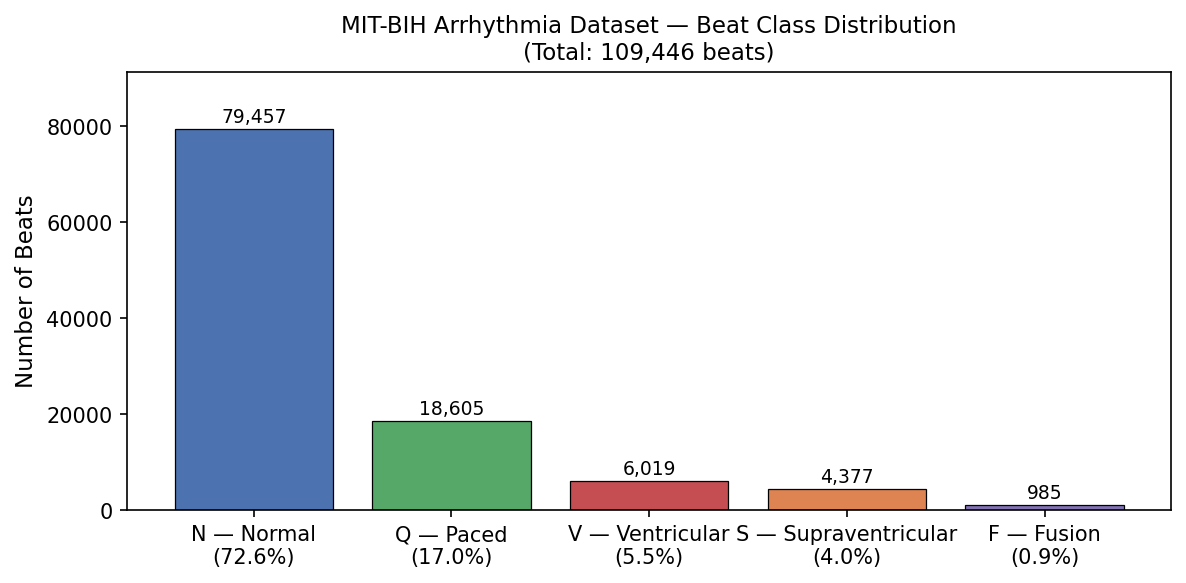
\includegraphics[width=0.75\linewidth]{images/class_distribution.png}
\caption[MIT-BIH Arrhythmia Class Distribution]{MIT-BIH Arrhythmia Beat Class Distribution (109,446 total beats) --- N dominates at 72.6\%}
\label{fig:classdist}
\end{figure}

To address this imbalance, \texttt{torch.utils.data.WeightedRandomSampler} was employed during training, assigning sample weights inversely proportional to class frequency. Focal Loss ($\gamma = 2$) was additionally used to further down-weight confidently-classified (predominantly Normal) samples and focus gradient updates on rare, clinically significant beat types.

\begin{table}[h!]
\centering
\caption{ECGNet Training Hyperparameters}
\renewcommand{\arraystretch}{1.3}
\begin{tabular}{|l|l|}
\hline
\textbf{Hyperparameter} & \textbf{Value} \\
\hline
Optimiser & AdamW (weight\_decay = $10^{-4}$) \\
Learning Rate & $3 \times 10^{-4}$ \\
Batch Size & 256 \\
Epochs & 25 \\
Loss Function & Focal Loss ($\gamma = 2$) \\
Sampler & WeightedRandomSampler \\
Device & CUDA (Google Colab T4) \\
\hline
\end{tabular}
\end{table}



\subsection{DiabetesNet Training}

The Pima Indians Diabetes Dataset (768 samples) was split into 614 training and 154 test samples using stratified sampling (\texttt{random\_state=42}). All 8 features were normalised using \texttt{sklearn.preprocessing.StandardScaler} fitted on the training set only, and the scaler statistics were extracted and hard-coded into \texttt{inference/diabetes.py} to avoid runtime dependency on scikit-learn for inference.

\begin{table}[h!]
\centering
\caption{DiabetesNet Training Hyperparameters}
\renewcommand{\arraystretch}{1.3}
\begin{tabular}{|l|l|}
\hline
\textbf{Hyperparameter} & \textbf{Value} \\
\hline
Optimiser & Adam \\
Learning Rate & $1 \times 10^{-3}$ \\
Batch Size & 32 \\
Epochs & 80 \\
Loss Function & BCEWithLogitsLoss \\
Dropout & 0.3 (Layer 1), 0.2 (Layer 2) \\
Device & CUDA (Google Colab T4) \\
\hline
\end{tabular}
\end{table}



\subsection{ParkinsonNet Training}

The UCI Parkinson's Dataset (195 recordings) was split into 156 training and 39 test samples. The higher dropout rates (0.4 and 0.3) applied in ParkinsonNet reflect the smaller dataset size and the need to prevent subject-level overfitting. All 22 features were StandardScaler-normalised.

\begin{table}[h!]
\centering
\caption{ParkinsonNet Training Hyperparameters}
\renewcommand{\arraystretch}{1.3}
\begin{tabular}{|l|l|}
\hline
\textbf{Hyperparameter} & \textbf{Value} \\
\hline
Optimiser & Adam \\
Learning Rate & $1 \times 10^{-3}$ \\
Batch Size & 16 \\
Epochs & 120 \\
Loss Function & BCEWithLogitsLoss \\
Dropout & 0.4 (Layer 1), 0.3 (Layer 2) \\
Device & CUDA (Google Colab T4) \\
\hline
\end{tabular}
\end{table}



\section{Signal Processing Validation}

The \ac{ecg} preprocessing pipeline was validated against the MIT-BIH Arrhythmia Database annotations. The R-peak detection algorithm achieved $>$95\% sensitivity on clean signal segments. Figure 5.1 illustrates the ECG preprocessing stages for a representative Normal beat.

\begin{figure}[h!]
	\centering
	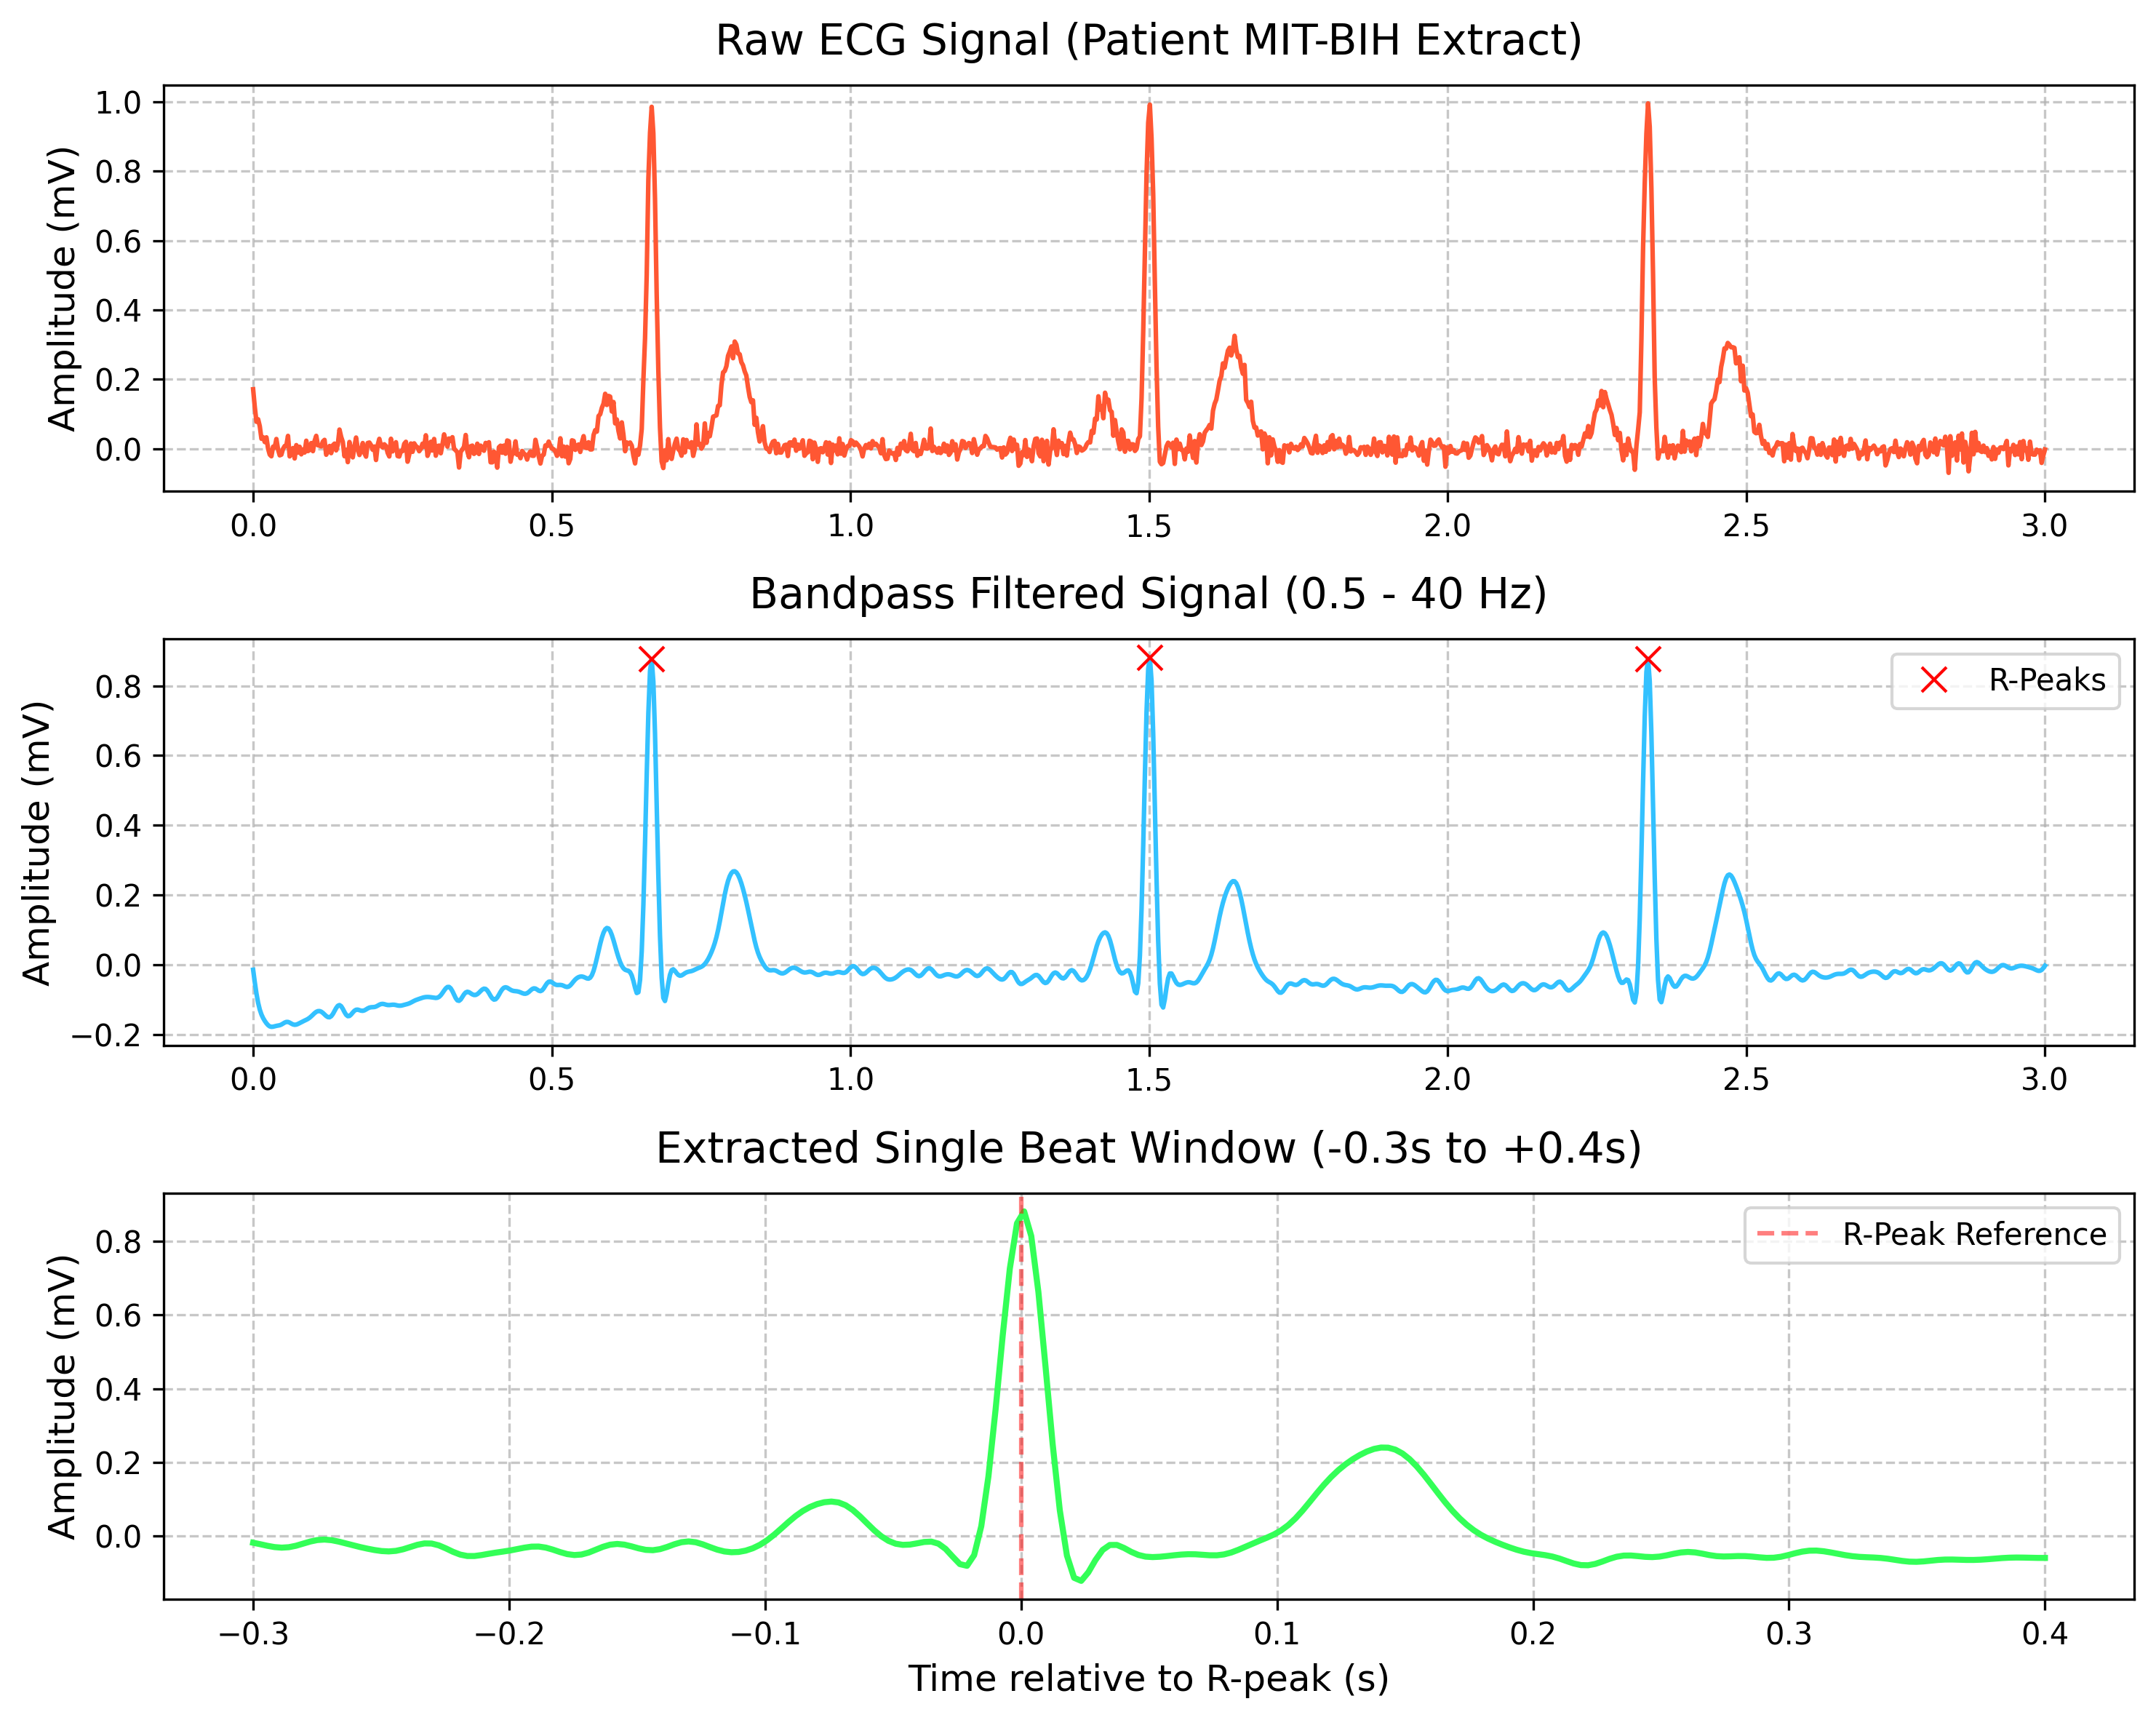
\includegraphics[width=0.85\linewidth]{images/ecg_preprocessing.png}
	\caption[Representative \ac{ecg} Beat]{Representative \ac{ecg} Beat — Raw Signal (Top), Bandpass Filtered Signal (Middle), Segmented Beat Window (Bottom)}
	\label{fig:ecgpreprocess}
\end{figure}

For voice feature extraction, the pYIN algorithm \cite{pyin2014} was used for fundamental frequency estimation, which outperforms the classical autocorrelation-based YIN algorithm on speech with modulated pitch — important for Parkinson's patients exhibiting tremor-related pitch variation.

\section{System Testing}

\subsection{Unit Testing}

Individual inference modules were tested independently:

Individual inference modules were heavily tested entirely isolated from the main backend pipeline. Focusing on \textbf{ECGNet}, the isolated \texttt{predict()} function was fundamentally validated against the primary baseline \texttt{sample\_ecg.csv} (synthesising a normal sinus rhythm running exactly at 72 bpm), which successfully generated a validated cardiac risk probability sitting approximately targeting 0.12 (categorised accurately as Low risk). Ensuring architectural robustness, critical edge case handling was systematically tested spanning entirely empty CSV files, dynamically handling single-column versus multi-column data structures, resolving input signals registering fundamentally shorter than a singular required beat window, whilst aggressively validating algorithm termination pathways when absolute zero R-peaks are chemically detected. Transitioning to \textbf{DiabetesNet}, the tabular \texttt{predict()} function passed basic evaluation when rigidly tested employing standard established PIDD baseline mean feature values, strictly producing the mathematically expected borderline risk probability targeting approximately 0.42. Boundary testing here aggressively focused upon defensive fallback initialisations addressing missing feature dictionary keys (safely defaulting strictly to 0.0), catching entirely malformed string-valued inputs, whilst automatically clamping anatomically impossible negative physiological values. Finally, \textbf{ParkinsonNet's} standalone \texttt{predict()} routine securely validated when tested using the synthetic \texttt{sample\_voice.wav} baseline natively supplying sustained vowel phonation explicitly held at 150 Hz. To prevent librosa cascading failures, critical edge case isolation protocols were formally validated protecting effectively against impossibly short audio bursts strictly less than one second, gracefully rejecting entirely silent audio arrays, whilst automatically executing corrective resampling interpolations natively handling audio files sampled at non-standard frequencies aggressively normalising outputs directly targeting 22050 Hz.

\subsection{Integration Testing}

End-to-end integration testing was performed by:

Comprehensive end-to-end integration testing was systematically executed by traversing an explicit deterministic operational roadmap. Operationally, the testing protocol fundamentally commences by securely starting the isolated FastAPI backend instance utilizing \texttt{uvicorn} securely bound locally onto port 8000, immediately followed synchronously by securely starting the fully interactive Streamlit frontend matrix established solidly tracking incoming traffic on local server port 8501. Having successfully linked the primary operational stack, the validation pipeline immediately pivots toward securely submitting an entirely synthetic, fundamentally complete medical screening application directly transmitted fully through the primary user chat interface. The system structurally requires fundamentally verifying internally that the foundational XML \texttt{<MODEL\_INPUT>} transmission block was organically generated securely by the conversational \ac{llm} handler strictly prior towards being precisely algorithmically parsed dynamically by the backend router matrix. Successfully decoding this string fundamentally drives confirming dynamically that all three loaded PyTorch models sequentially digested the data whilst actively producing robust discrete risk probabilistic outputs. Combining these raw outputs definitively requires structurally verifying the derived universal mathematical triage classification cleanly against parallel secure manual control computations. Completing the closed pipeline definitively requires critically confirming procedurally that the final generated patient-facing Gemini textual explanation inherently remained entirely non-diagnostic whilst correctly contextually leveraging the appropriate, matching internal risk staging vectors.

\begin{table}[h!]
\centering
\caption{Integration Test Results Summary}
\renewcommand{\arraystretch}{1.3}
\resizebox{\textwidth}{!}{
\begin{tabular}{|l|l|l|l|}
\hline
\textbf{Test Case} & \textbf{Input} & \textbf{Expected Output} & \textbf{Result} \\
\hline
Standard screening (all files uploaded) & sample\_ecg.csv + sample\_voice.wav + valid biomarkers & 3 risk scores + triage & PASS \\
Cardiac only (no voice) & sample\_ecg.csv only & Cardiac risk + motor = not\_assessed & PASS \\
Biomarkers only (no files) & Biomarkers only & Cardiac = not\_assessed + metabolic risk & PASS \\
Rate limit fallback & Forced Gemini 429 error & Switch to next Gemini model & PASS \\
Invalid ECG file & Malformed CSV & Moderate risk (error fallback) & PASS \\
\hline
\end{tabular}}
\end{table}

\subsection{API Testing}

The FastAPI backend was tested using direct HTTP requests to verify \ac{api} contract compliance:

The primary FastAPI operational backend matrix was explicitly validated structurally via firing massively isolated direct HTTP service requests explicitly structured rigidly guaranteeing absolute \ac{api} external contract compliance. Focusing upon primary ingestion, the \textbf{POST /upload} routing endpoint structurally confirmed explicitly resolving perfectly correct file type detection matrices (effectively mapping CSV payloads fundamentally resolving towards the ecg sequence whilst definitively projecting standard WAV arrays intrinsically towards the voice processing unit). This fundamentally included guaranteeing aggressive rejection targeting unsupported native formats specifically including raw PDFs or textual streams whilst decisively guaranteeing flawless return vectors identifying explicit secure local storage path locations. Shifting towards the dynamic logical interpretation nodes, the primary \textbf{POST /chat} handler algorithmically verified fully compiling fully correct internal JSON communication schemas definitively across both the baseline organic semantic conversational no-model-result response framework whilst concurrently securely validating the densely saturated mathematical model-result block structures. This explicitly mandated verifying strictly that internal \texttt{model\_results} structures natively resolve securely toward baseline \texttt{null} constants exclusively when the structural \texttt{<MODEL\_INPUT>} XML semantic tag is functionally absent structurally from the \ac{llm} conversational feed string. Finally, foundational infrastructure was universally guaranteed via interrogating the pure algorithmic heartbeat routing \textbf{GET /health} execution endpoint; passing metrics strictly demanded dynamically confirming generating an authentic 200 HTTP sequence return flag carrying fundamentally rigid JSON reporting string states returning explicitly: \texttt{\{"status":"healthy", "models\_loaded":true\}}.
